\section{Theoretische Grundlagen}
    \subsection{Erzeugung instabiler Kerne mit Neutronen}
        Um Zefallsprozesse hervorzurufen, werden Atome mit Neutronen beschossen. Dabei dringt das Neutron, ohne die Coulomb-Barriere überwinden zu müssen, in den Kern des beschossenen Atoms ein. 
        Der um ein Neutron erweiterter Kern $A^*$ heißt Zwischenkern und ist um die kinetische- sowie Ruheenergie des Neutrons energiereicher im Vergleich zu seinem Vorgänger. Der nun angeregte Kern
        gibt die übrige Energie über ein Photon ab und befindet sich nun wieder im Grundzustand $A$.
        
        \begin{equation*}
            \ce{^{m}_{z}A} + \ce{^{1}_{0}n} \longrightarrow \ce{^{m+1}_{z}A}^* \longrightarrow \ce{^{m+1}_{z}A} + \gamma
        \end{equation*}

        \noindent
        Der so neu entstandene Kern ist aufgrund der höheren Neutronenzahl häufig instabil und wird daher zerfallen. Dies geschieht durch den $\beta^-$-Zerfall, bei dem der instabile Kern in einen
        stabilen Kern übergeht und dabei ein Elektron e, ein Antielektronneutrino $\bar{\nu_e}$ sowie deren kinetische Energie freigesetzt wird. Die kinetische Energie entspringt der Massendifferenz
        (Massendeffekt) beim $\beta^-$-Zerfall mit $\Delta E = \Delta mc^2$.

        \begin{equation*}
            \ce{^{m+1}_{z}A} \longrightarrow \ce{^{m+1}_{z+1}C} + \text{e} + \text{E}_{\text{Kin}} + \bar{\nu_e}
        \end{equation*}

    \subsection{Aufnahme von Neutronen}
        Die Wahrscheinlichkeit, dass ein Neutron in einen Kern eindringt wird durch den Wirkungsquerschnitt quantifiziert, dessen Einheit dem barn entspricht ($1 \text{barn} \equiv 10^{-24} cm^2$)
        und der bei einer 1 $cm^2$ großen Folie über folgende Formel berechnet wird
        
        \begin{equation*}
            \sigma = \frac{\text{u}}{\text{nKd}}
        \end{equation*}

        \noindent
        Dabei steht u für die Anzahl an Neutroneneinfängen, n für die Anzahl an einfallendne Neutronen, d für die Dicke des Schirmmaterials und K für die Anzahl der Atome pro Volumen in $cm^{-3}$.
        Da der Wirkungsquerschnitt für das Eindringen eines Neutrons geschwindigkeitsabhängig ist, wird bei der Berechnung zwischen schnellen und langsammen Neutronen unterschieden. Diese 
        Unterscheidung erfolgt über die ebenfalls geschwindigkeitsabhängige De-Broglie-Wellenlänge:

        \begin{equation*}
            \lambda = \frac{\text{h}}{m_{\text{Neutron}} \cdot v_{\text{Neutron}}}
        \end{equation*}

        \noindent

        \subsubsection*{Schnelle Neutronen}
            Es handelt sich um schnelle Elektronen, wenn deren Geschwindigkeit so groß ist, dass deren De-Broglie-Wellenlänge gegenüber dem Kernradius ($\approx 10^{-12}$cm) klein wird. Dabei 
            lässt sich das System analog zur Streuung von Licht an einem makroskopischen Objekt betrachten.

        \subsubsection*{Langsame Neutronen}
            Interessanter ist der Fall langsammer Neutronen, bei denen die De-Broglie-Wellenlänge groß gegen den Kernradius ist. Hierbei kann der Wirkungsquerschnitt in Abhängigkeit von der 
            der Energie des Neutrons und den Energieniveaus des Zwischenkerns berechnen. $\widetilde{c}$ und $\sigma_0$ sind dabei Konstanten der zugehörigen Kernreaktion.

            \begin{align*}
                \sigma(\text{E}) &= \sigma_0 \cdot \sqrt{\frac{\text{E}_{\text{r}_i}}{\text{E}}} \cdot \frac{\widetilde{c}}{\left(\text{E} - \text{E}_{\text{r}_i}\right)^2 + \widetilde{c}}\\
                \text{E} &= \frac{1}{2} \cdot m_{\text{Neutron}} \cdot v_{\text{Neutron}}^2
            \end{align*}

            \noindent
            Wenn nun die Energie des einfallenden Teilchens viel kleiner ist als die des jeweiligen Energieniveaus des Kerns ist der Wirkungsquerschnitt proportional zum Kehrwert der Wurzel der
            Neutronenenergie und somit zum Kehrwert der Geschwindigkeit des Neutrons. Da zur Aktivierung der Kerne ein möglichst hoher Wirkungsquerschnitt gewünscht ist, werden langsamme und
            niederenergetische Neutronen bevorzugt.

    
    \subsection{Erzeugung niederenergetischer Neutronen}
        Neutronen sind ungebunden instabil und kommen daher nicht natürlich im freiem Zustand vor. Die für den Neutroneneinfang vorgesehenen Neutronen werden daher durch den Beschuss von 
        Beryllium mit Alpha-Teilchen erzeugt.

        \begin{equation*}
            \ce{^{9}_{4}Be} + \ce{^{4}_{2}He} \longrightarrow \ce{^{12}_{6}C} + \ce{^{1}_{0}n}
        \end{equation*}

        \noindent
        Die dabei freigesetzten Neutronen haben jedoch eine kontinuierliche Energieverteilung mit bis zu 13,7 MeV und sind damit nicht niederenergetisch. Daher wird die Quelle von einer 
        Materieschicht umhüllt. Wenn die Neutronen in diese eintreten kommt es solange zu elastischen Stößen bis die kinetische Energie der der umgebenden Moleküle entspricht. Dann beträgt
        die Neutronenenergie, der nun als thermische Neutronen bezeichneten Neutronen, etwa 0,025 eV, was einer Temperatur der Teilchenmenge von 290 Kelvin entspricht. Dieser Prozess läuft 
        umso schneller ab, desto ähnlicher sich die Massen der Stoßpartner sind. Dies lässt sich aus Gleichung \ref{eqn:Stoß} lesen. Diese gibt die pro Stoß übergebende Energie in Abhängigkeit
        von der Anfangsenergie $\text{E}_0$ und den Massen der verschiedenen Stoßpartner M und m an. Die kleinste Masse wäre bei Wasserstoff gegeben, sodass als Stoßpartner die Neutronen von
        Paraffin, das hauptsächlich aus Wasserstoff besteht, genutzt werden. 

        \begin{equation}
            \text{E}_{\text{ü}} = \text{E}_0 \cdot \frac{4\text{Mm}}{\left(M + m\right)^2}
            \label{eqn:Stoß}
        \end{equation}

    \subsection{Zerfallsgesetz}
        Gemäß dem Zerfallsgesetz radioaktiver Isotope ist die Anzahl der nach einer gewissen Zeit t von der Ausgangsanzahl $\text{N}_0$ an vorhandenen Teilchen noch übrige Teilchenzahl N
        über folgende Formel berechenbar. Dabei steht $\lambda$ für die Zerfallskonstante.
        
        \begin{equation}
            \text{N}(t) = \text{N}_0 \cdot e^{-\lambda t}
            \label{eqn:Zerfallsgesetz}
        \end{equation}

        \noindent
        Die Halbwertszeit beschreibt die Dauer in der von der anfänglichen Teilchenzahl nur noch die Hälfte übrig ist. Dies lässt sich wie folgt ausdrücken.

        \begin{equation}
            \frac{1}{2} \cdot \text{N}_0 = \text{N}_0 \cdot e^{-\lambda T_{\frac{1}{2}}} \qquad \longrightarrow \qquad T_{\nicefrac{1}{2}} = \frac{\ln(2)}{\lambda}
            \label{eqn:Halbwertszeit}
        \end{equation}

        \noindent
        So kann die spezifische Halbwertszeit für die Isotope bestimmt werden.
        Da die Anzahl der vorhandenen Kerne jedoch nur umständlich zu bestimmen ist, wird die Zerfallskonstante stattdessen über die Anzahl der zerfallenden Kerne pro Zeitintervall $N_{\Delta t}$
        bestimmt, da diese Zerfälle einfacher detektiert werden können. Die Anzahl der zerfallenden Kerne ergibt sich durch Subtraktion der nach einem Intervall $\Delta t$ vorhandenen Kernen von
        den vor diesem Intervall vorhandenen Kernen.

        \begin{equation*}
            \text{N}_{\Delta t}(t) = \text{N}(t) - \text{N}(t + \Delta t)
        \end{equation*}

        \noindent
        Anwenden des Zerfallsgesetzes \ref{eqn:Zerfallsgesetz} und anschließendes anwenden des natürlichen Logarithmus liefert eine weitere Möglichkeit zur Bestimmung der Halbwertszeit.
        
        \begin{equation}
            \text{N}_{\Delta t}(t) = \text{N}_0 \cdot e^{-\lambda t} - \text{N}_0 \cdot e^{-\lambda (t + \Delta t)} = \text{N}_0 \cdot \left(1 - e^{-\lambda \Delta t}\right) \cdot e^{-\lambda t}
            \label{eqn:Zerfallsgesetz_}
        \end{equation}
            
        \begin{equation}
            \ln\left(\text{N}_{\Delta t}(t)\right) = \ln \left(\text{N}_0 \cdot \left(1 - e^{-\lambda \Delta t}\right)\right) - \lambda t
            \label{eqn:theorieGerade}
        \end{equation}
        
        \noindent
        Auf der echten Seite dieser Gleichung ist allein t variabel und auf der linken Seite $N_{\Delta t}$, sodass die Zerfallskonstante über eine lineare Regression bestimmbar ist und daraus 
        wiederum die Halbwertszeit berechnet werden kann. Dabei muss
        $\Delta t$ exakt gewählt sein, da zu kleine Werte zu große statistische Fehler mit sich bringen und zu große Zeiten, die gegen die Halbwertszeit laufen einen systematoschen Fehler mit
        sich bringen.

    \subsection{Besonderheiten des Experiments}
        Die Bestimmung der Halbwertszeit soll für zwei Elemente durchgeführt werden.

            \subsubsection*{Vanadium}
            Das durch Neutroneneinfang aktivierte Vanadium zefällt wiefolgt:

            \begin{equation*}
                \ce{^{51}_{23}V} + \ce{^{1}_{0}n} \longrightarrow \ce{^{52}_{23}V}  \longrightarrow \ce{^{52}_{24}Cr} + \text{e} + \bar{\nu_e}
            \end{equation*}

            \noindent 
            Es entsteht nur ein instabiles Isotop und die Bestimmung über eine Ausgleichsgerade lässt sich problemlos durchführen.
            
            \subsubsection*{Rhodium}
            Im Gegensatz zum Vanadium entstehen bei Rhodium durch Neutroneneinfang zwei instabile Isotope mit verschiedener Wahrscheinlichkeit.

            \begin{equation}
                \ce{^{103}_{45}Rh} + \ce{^{1}_{0}n}  \begin{cases}
                    \xrightarrow{10\%} \ce{^{104i}_{45}Rh} \longrightarrow \ce{^{104}_{45}Rh} + \gamma \longrightarrow \ce{^{104}_{46}Pd} + \text{e} + \bar{\nu_e} \\
                    \xrightarrow{90\%} \ce{^{104}_{45}Rh} \longrightarrow \ce{^{104}_{46}Pd} + \text{e} + \bar{\nu_e}
                \end{cases}
                \label{eqn:Rhodium}
            \end{equation}

            \noindent
            Diese Isotope zerfallen auch beide in andere Elemente. Gemessenen werden kann jedoch nur die Gesamtaktivität der beiden Zerfallsketten. Da die beiden Isotope unterschiedlich schnell 
            zerfallen ist nach einer gewissen Zeit $t^*$ nur noch das langlebige Isotop für die Aktivität verantwortlich. So kann für den Graphen der Messwerte eine lineare Regression für den 
            Bereich $t>t^*$ angefertigt und damit die Zerfalsskonstante des langlebigen Isotops bestimmt werden. Durch Abziehen diesen Untergrunds von dem Messwerten und anschließender linearen 
            Regression über den Bereich $t<t^*$ kann dann die Zerfallskonstante des kurzlebigen Isotops bestimmt werden. Die beim Zefall von $\ce{^{104i}_{45}Rh}$ frei werdende Gamma-Strahlung
            muss nicht berücksichtigt werden, da sie nur geringfügig zur gesamten Zählung beiträgt. 

            \FloatBarrier

            \begin{figure}[h]
                \centering
                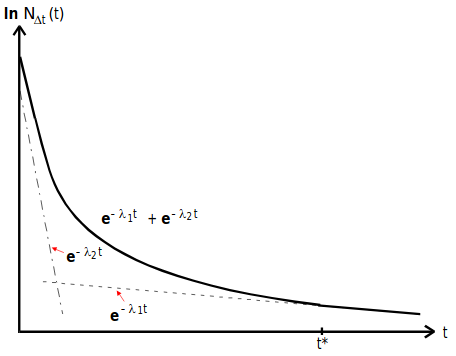
\includegraphics[width = 0.6\textwidth]{pictures/RhSchema.png}
                \caption{In der Abbildung ist eine schematische Darstellung der Zerfallskurve zweier Isotope, deren Halbwertszeiten stark verschieden sind. Die Anzahl der zerfallenden Kerne ist dabei logarithmisch gegen die Zeit aufgetragen. Die Zerfallskurve eines einzelnen Isotops würde linear verlaufen und das tun auch die linearen Regressionen der einzelnen Isotope (gestrichelt)  [1]}
                \label{fig:RhSchema}
            \end{figure}

            \FloatBarrier
